Метод анализа КДО по прежнему являются одним из основных инструментов диагностики не только совершенства
кристаллических материалов \cite{sov_1} - \cite{sov_5}, в частности, объемных и поверхностных дефектов в
монокристаллах, тонких пленках, а также многослойных кристаллических структурах, но и для анализа физических
процессов происходящих в кристаллах, таких как воздействие внешнего электрического поля \cite{piezo102} (пьезоэлектрический эффект),
 температуры \cite{temp} или влияние магнитного поля.

Измерение кривой дифракционного отражения в двухкристальной схеме представляет
собой измерение зависимости отраженного образцом рентгеновского излучения при
пошаговом повороте исследуемого кристалла относительно падающего на него
излучения в окрестности точного значения угла Брэгга.
Существует несколько схем измерения кривых отражения рентгеновского излучения.

\subsubsection*{$\omega$ - сканирование}
В данном типе сканирования кривая отражения измеряется путем поворота образца
относительно падающего пучка в плоскости дифракции. При таком сканировании
угол между падающим и дифрагированным пучками (угол рассеяния) остается постоянным
(рис. \ref{ris:omega_scan}). Получаемая в результате кривая носит название кривой качания.


\begin{figure}[H]
  \centering
  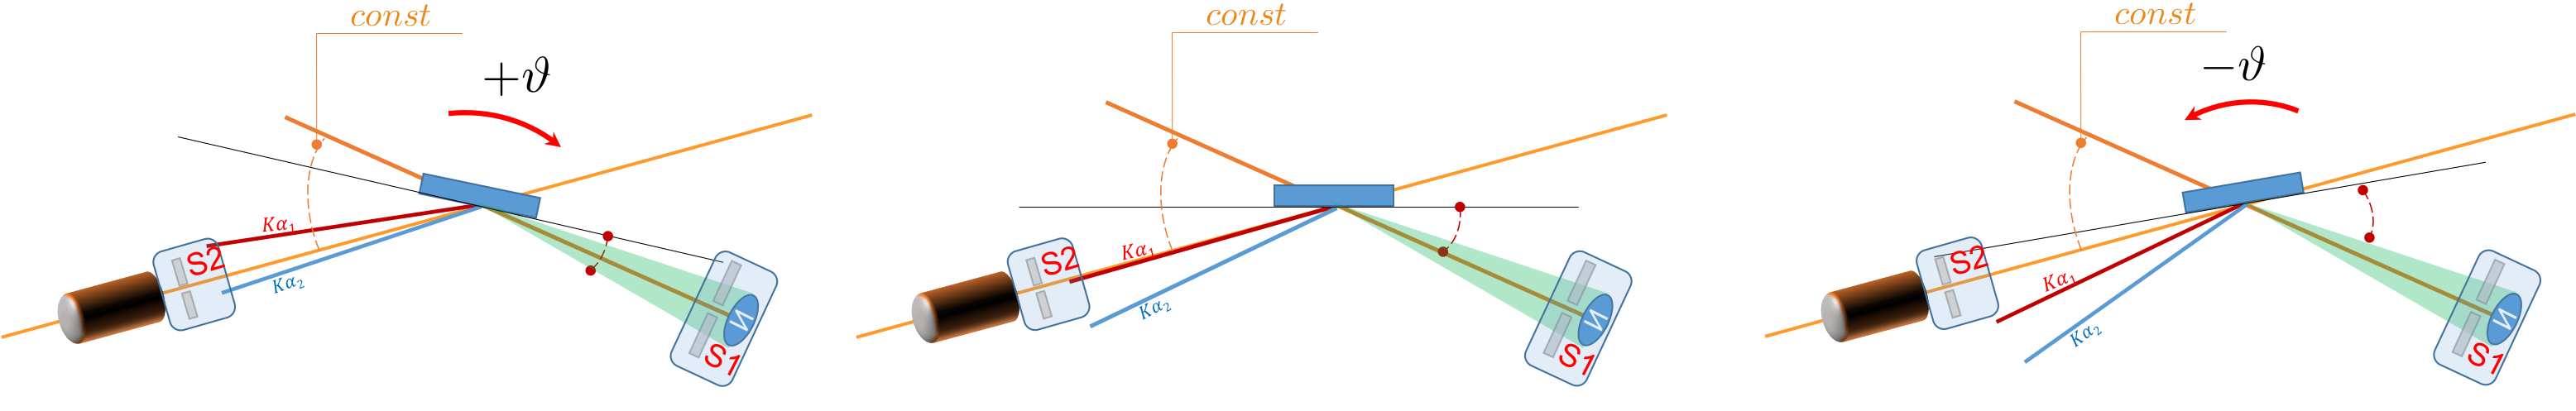
\includegraphics[width=1\textwidth]{images/omega_scan.png}
  \caption{Схема реализации $\omega $ - сканирования}
  \label{ris:omega_scan}
\end{figure}

\subsubsection*{$\vartheta - 2\vartheta$ - сканирование}
В отличие от предыдущего, данный метод сканирования соответствует изменению
 модуля вектора рассеяния при неизменном его угловом положении
 (рис. \ref{ris:theta_2theta_scan}). Угловое положение падающего пучка и
 детектора изменяется синхронно и симметрично относительно используемой системы
 атомных плоскостей, а установленная перед детектором апертурная щель вырезает
  только зеркально отраженную часть пучка. Именно поэтому при построении карт
   пространственного распределения спектра полосы щелей на этих картах остаются
   неподвижными (т.к. несмотря на движение щели  $S_2$ в процессе
    $\vartheta - 2\vartheta$ -  сканирования ее отстройка от зеркального
    положения всегда равна 0).

 \begin{figure}[H]
   \centering
   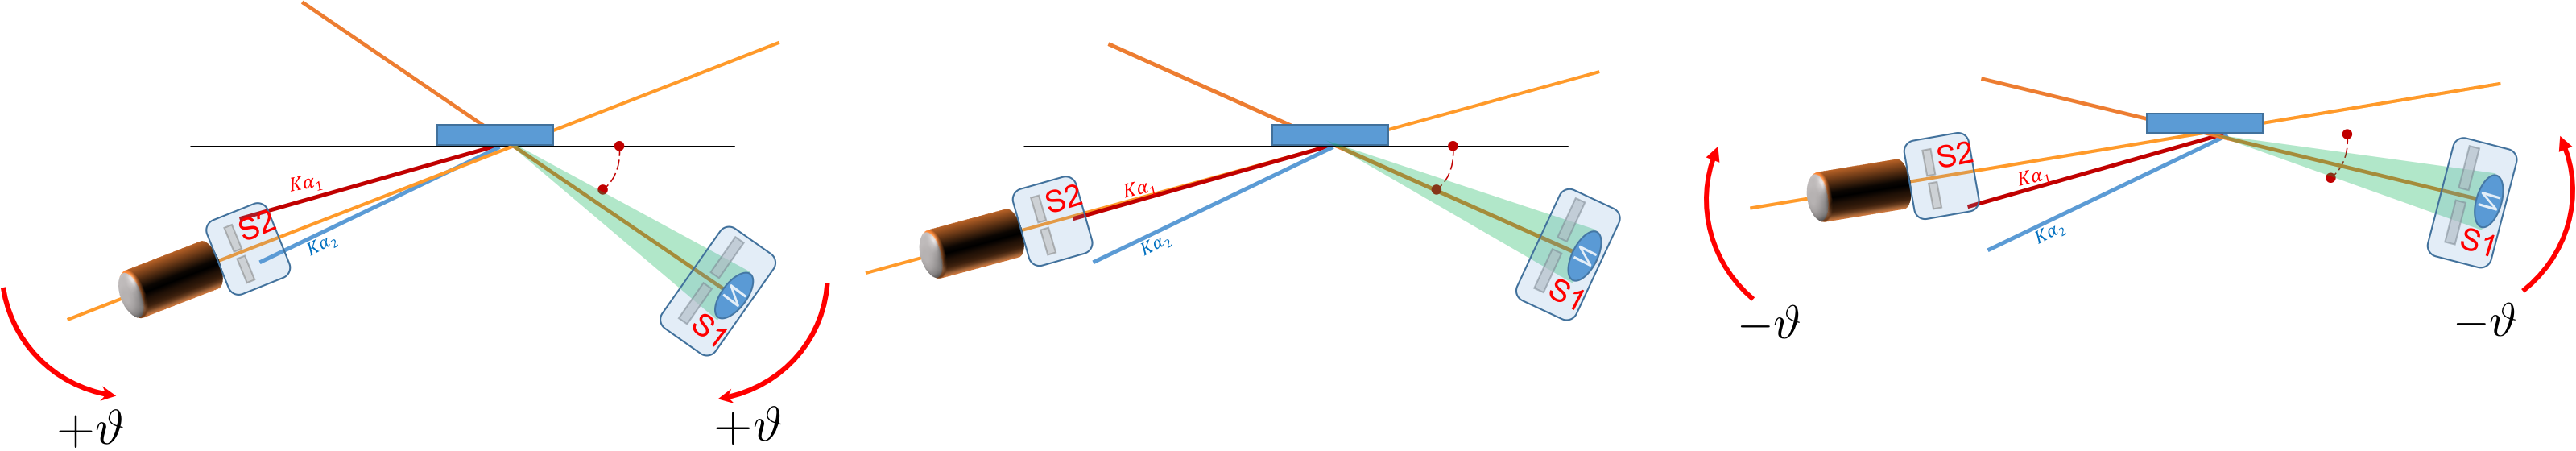
\includegraphics[width=1\textwidth]{images/theta_2theta_scan.png}
   \caption{Схема реализации $\vartheta - 2\vartheta$ - сканирования}
   \label{ris:theta_2theta_scan}
 \end{figure}
Кроме того, используемый подход основанный на спектрально-угловом представлении
для данного типа сканирования, наглядно демонстрирует интересный эффект.
 Независимо от ширины входной и приемной щелей характеристическая линия спектра
 трубки $k_{\alpha 2}$ всегда вносит вклад в КДО, проявляясь в виде дополнительного
 пика на ее хвосте, что будет показано далее.
